
\section{Motivation}
\label{sec:motivation}

\subsection{An example of a commit }
\label{sec:examle}

\subsection{Convolutional Neural Networks}
\label{sec:background_cnn}
\begin{figure*}[t!]
\center
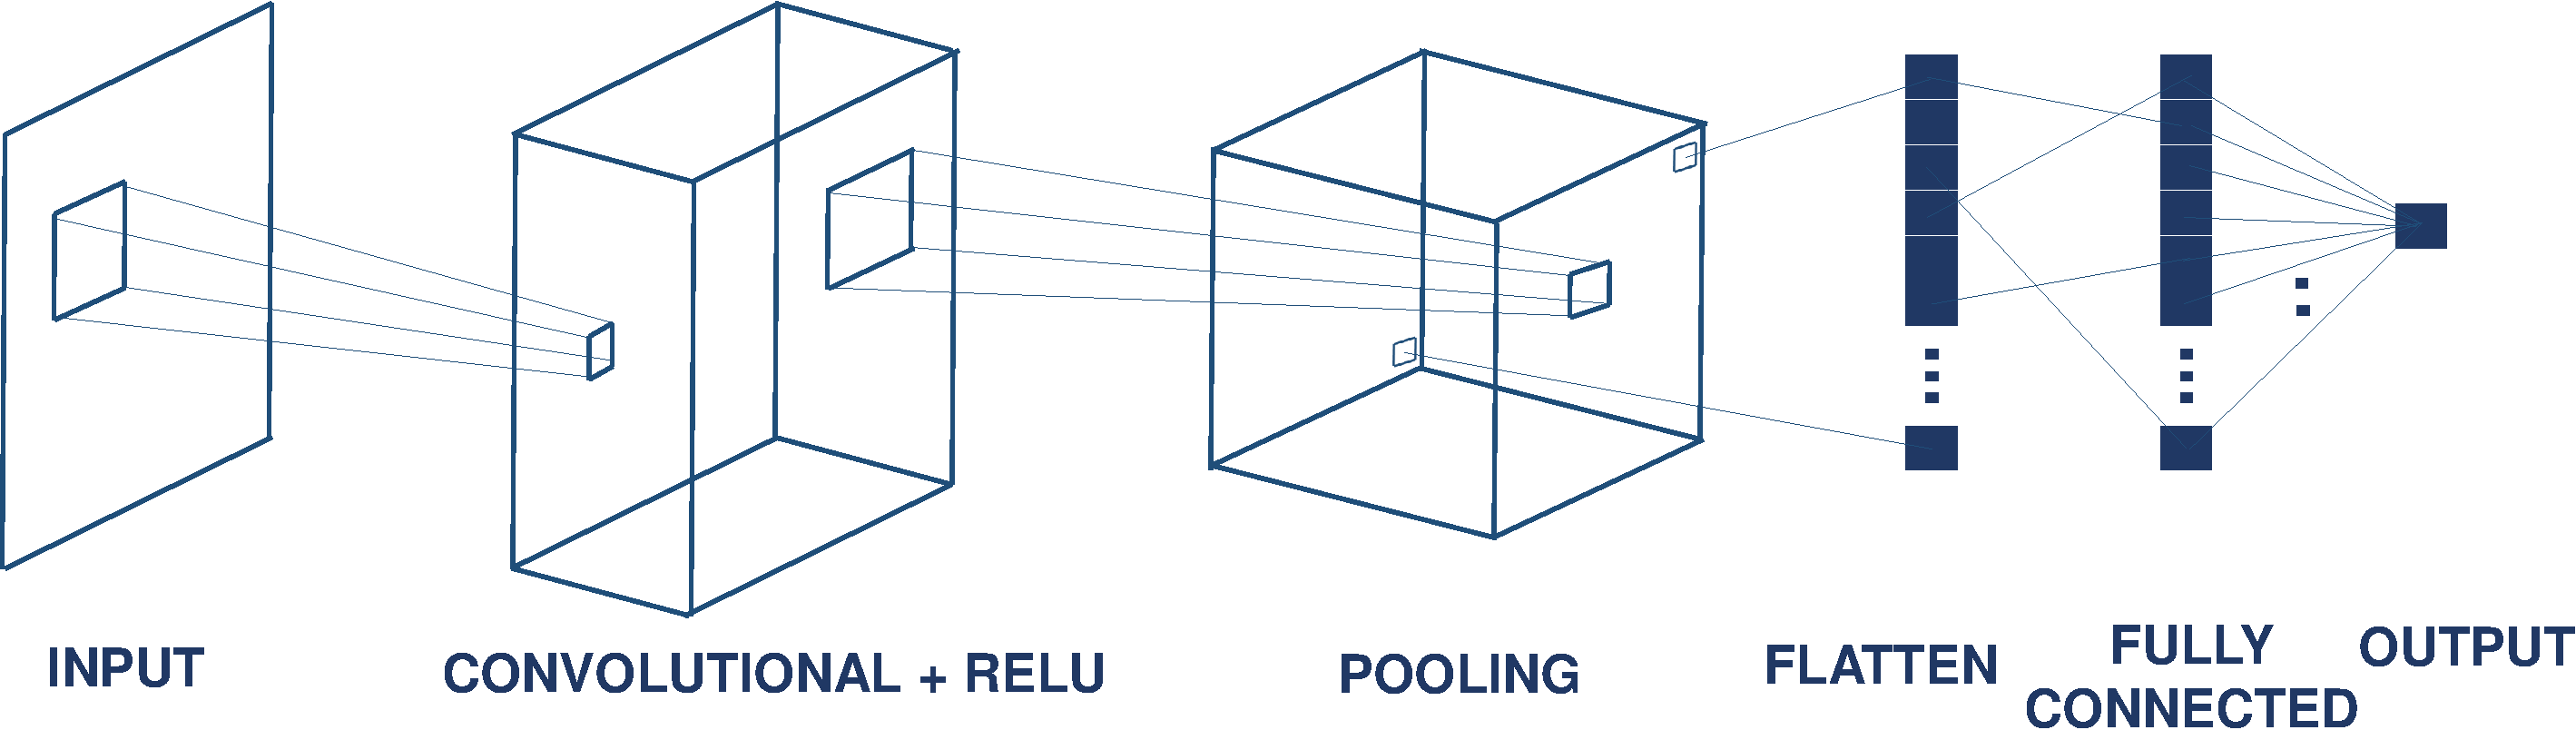
\includegraphics[scale=0.3]{figs/cnn.pdf}
\caption{A simple convolutional neural network architecture.}
\label{fig:cnn}
\end{figure*}

One of the most powerful forms of deep learning neural networks is the Convolutional Neural Network (CNN)~\cite{lecun2015deep}. CNNs are widely used to solve image pattern recognition problems and have been achieved significant results~\cite{karpathy2014large, lawrence1997face, krizhevsky2012imagenet}. Like traditional deep learning networks, CNNs receive an input and perform a product operation followed by a nonlinear function. The last layer is the output layer containing objective functions~\cite{zhao2017loss} associated with the labels of the input.



